\documentclass[tikz]{standalone}

\usepackage{tikz}

\begin{document}

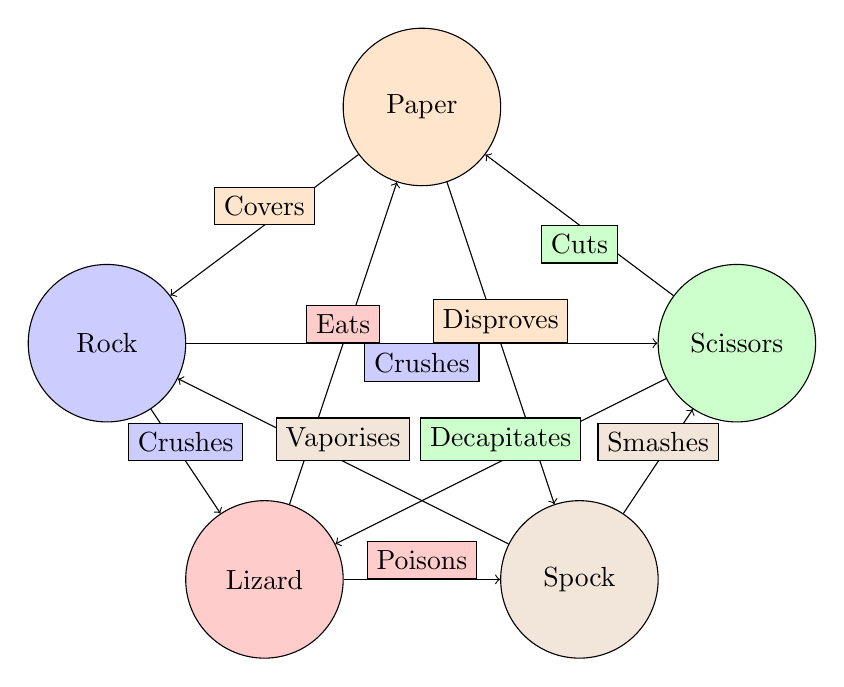
\begin{tikzpicture}

\node (R) at (0,0) [circle, minimum width = 2cm, draw, fill=blue!20] {Rock};
\node (P) at (4,3) [circle, minimum width = 2cm, draw, fill=orange!20] {Paper};
\node (S) at (8,0) [circle, minimum width = 2cm, draw, fill=green!20] {Scissors};
\node (Lz) at (2,-3) [circle, minimum width = 2cm, draw, fill=red!20] {Lizard};
\node (Sp) at (6,-3) [circle, minimum width = 2cm, draw, fill=brown!20] {Spock};

\draw [->] (P) -- node[above, fill=orange!20, draw] {Covers} (R);
\draw [->] (P) -- node[above, fill=orange!20, draw] {Disproves} (Sp);

\draw [->] (R) -- node[below, fill=blue!20, draw] {Crushes} (S);
\draw [->] (R) -- node[above, fill=blue!20, draw] {Crushes} (Lz);

\draw [->] (S) -- node[below, fill=green!20, draw] {Cuts} (P);
\draw [->] (S) -- node[above, fill=green!20, draw] {Decapitates} (Lz);

\draw [->] (Lz) -- node[above, fill=red!20, draw] {Eats} (P);
\draw [->] (Lz) -- node[above, fill=red!20, draw] {Poisons} (Sp);

\draw [->] (Sp) -- node[above, fill=brown!20, draw] {Vaporises} (R);
\draw [->] (Sp) -- node[above, fill=brown!20, draw] {Smashes} (S);
\end{tikzpicture}
\end{document}
